\documentclass[
  man,
  longtable,
  nolmodern,
  notxfonts,
  notimes,
  colorlinks=true,linkcolor=blue,citecolor=blue,urlcolor=blue]{apa7}

\usepackage{amsmath}
\usepackage{amssymb}
\usepackage{setspace}



\RequirePackage{longtable}
\RequirePackage{threeparttablex}

\usepackage{framed}


\makeatletter
\renewcommand{\paragraph}{\@startsection{paragraph}{4}{\parindent}%
	{0\baselineskip \@plus 0.2ex \@minus 0.2ex}%
	{-.5em}%
	{\normalfont\normalsize\bfseries\typesectitle}}

\renewcommand{\subparagraph}[1]{\@startsection{subparagraph}{5}{0.5em}%
	{0\baselineskip \@plus 0.2ex \@minus 0.2ex}%
	{-\z@\relax}%
	{\normalfont\normalsize\bfseries\itshape\hspace{\parindent}{#1}\textit{\addperi}}{\relax}}
\makeatother




\usepackage{longtable, booktabs, multirow, multicol, colortbl, hhline, caption, array, float, xpatch}
\usepackage{subcaption}


\renewcommand\thesubfigure{\Alph{subfigure}}
\setcounter{topnumber}{2}
\setcounter{bottomnumber}{2}
\setcounter{totalnumber}{4}
\renewcommand{\topfraction}{0.85}
\renewcommand{\bottomfraction}{0.85}
\renewcommand{\textfraction}{0.15}
\renewcommand{\floatpagefraction}{0.7}

\usepackage{tcolorbox}
\tcbuselibrary{listings,theorems, breakable, skins}
\usepackage{fontawesome5}

\definecolor{quarto-callout-color}{HTML}{909090}
\definecolor{quarto-callout-note-color}{HTML}{0758E5}
\definecolor{quarto-callout-important-color}{HTML}{CC1914}
\definecolor{quarto-callout-warning-color}{HTML}{EB9113}
\definecolor{quarto-callout-tip-color}{HTML}{00A047}
\definecolor{quarto-callout-caution-color}{HTML}{FC5300}
\definecolor{quarto-callout-color-frame}{HTML}{ACACAC}
\definecolor{quarto-callout-note-color-frame}{HTML}{4582EC}
\definecolor{quarto-callout-important-color-frame}{HTML}{D9534F}
\definecolor{quarto-callout-warning-color-frame}{HTML}{F0AD4E}
\definecolor{quarto-callout-tip-color-frame}{HTML}{02B875}
\definecolor{quarto-callout-caution-color-frame}{HTML}{FD7E14}

%\newlength\Oldarrayrulewidth
%\newlength\Oldtabcolsep


\usepackage{hyperref}
\usepackage[protrusion=true]{microtype}



\providecommand{\tightlist}{%
  \setlength{\itemsep}{0pt}\setlength{\parskip}{0pt}}
\usepackage{longtable,booktabs,array}
\usepackage{calc} % for calculating minipage widths
% Correct order of tables after \paragraph or \subparagraph
\usepackage{etoolbox}
\makeatletter
\patchcmd\longtable{\par}{\if@noskipsec\mbox{}\fi\par}{}{}
\makeatother
% Allow footnotes in longtable head/foot
\IfFileExists{footnotehyper.sty}{\usepackage{footnotehyper}}{\usepackage{footnote}}
\makesavenoteenv{longtable}

\usepackage{graphicx}
\makeatletter
\newsavebox\pandoc@box
\newcommand*\pandocbounded[1]{% scales image to fit in text height/width
  \sbox\pandoc@box{#1}%
  \Gscale@div\@tempa{\textheight}{\dimexpr\ht\pandoc@box+\dp\pandoc@box\relax}%
  \Gscale@div\@tempb{\linewidth}{\wd\pandoc@box}%
  \ifdim\@tempb\p@<\@tempa\p@\let\@tempa\@tempb\fi% select the smaller of both
  \ifdim\@tempa\p@<\p@\scalebox{\@tempa}{\usebox\pandoc@box}%
  \else\usebox{\pandoc@box}%
  \fi%
}
% Set default figure placement to htbp
\def\fps@figure{htbp}
\makeatother


% definitions for citeproc citations
\NewDocumentCommand\citeproctext{}{}
\NewDocumentCommand\citeproc{mm}{%
  \begingroup\def\citeproctext{#2}\cite{#1}\endgroup}
\makeatletter
 % allow citations to break across lines
 \let\@cite@ofmt\@firstofone
 % avoid brackets around text for \cite:
 \def\@biblabel#1{}
 \def\@cite#1#2{{#1\if@tempswa , #2\fi}}
\makeatother
\newlength{\cslhangindent}
\setlength{\cslhangindent}{1.5em}
\newlength{\csllabelwidth}
\setlength{\csllabelwidth}{3em}
\newenvironment{CSLReferences}[2] % #1 hanging-indent, #2 entry-spacing
 {\begin{list}{}{%
  \setlength{\itemindent}{0pt}
  \setlength{\leftmargin}{0pt}
  \setlength{\parsep}{0pt}
  % turn on hanging indent if param 1 is 1
  \ifodd #1
   \setlength{\leftmargin}{\cslhangindent}
   \setlength{\itemindent}{-1\cslhangindent}
  \fi
  % set entry spacing
  \setlength{\itemsep}{#2\baselineskip}}}
 {\end{list}}
\usepackage{calc}
\newcommand{\CSLBlock}[1]{\hfill\break\parbox[t]{\linewidth}{\strut\ignorespaces#1\strut}}
\newcommand{\CSLLeftMargin}[1]{\parbox[t]{\csllabelwidth}{\strut#1\strut}}
\newcommand{\CSLRightInline}[1]{\parbox[t]{\linewidth - \csllabelwidth}{\strut#1\strut}}
\newcommand{\CSLIndent}[1]{\hspace{\cslhangindent}#1}





\usepackage{newtx}

\defaultfontfeatures{Scale=MatchLowercase}
\defaultfontfeatures[\rmfamily]{Ligatures=TeX,Scale=1}





\title{Necessary Condition Analysis With Psychological Data: A
Psychometric Critique}


\shorttitle{The bare necessity of NCA}


\usepackage{etoolbox}








\authorsnames{Tommaso Feraco,Enrico Toffalini}





\affiliation{
{Department of General Psychology, University of Padua}}




\leftheader{Feraco and Toffalini}



\abstract{This study evaluates the interpretability of Necessary
Condition Analysis (NCA) when applied to psychological data, where
variables typically represent latent constructs measured through
imperfect instruments. Using a unified simulation framework, we held the
latent relationship between two variables constant while systematically
varying common psychometric and sampling features, including score
construction, reliability, ordinal scaling and threshold placement,
skewness, and range restriction. Results indicate that NCA effect sizes
are highly sensitive to properties of the observed score distribution.
Substantial variability emerged across conditions despite identical
latent associations. In particular, ordinal scaling, threshold shifts,
and skewness consistently altered the geometry of the data space,
producing marked changes in estimated necessity effects. Reliability and
score construction also contributed to deviations, though to a lesser
extent. Range restriction further amplified discrepancies by modifying
both the latent and observed distributions. Crucially, NCA effect sizes
were also influenced by the sample size of the simulations. Overall,
observed-score NCA estimates frequently diverged from their latent
counterparts, suggesting that NCA in psychological applications
primarily reflects distributional features induced by measurement and
sampling rather than stable properties of underlying constructs. These
findings raise concerns about the substantive interpretation of
necessity claims in psychology and highlight the need for stronger
theoretical justification and more transparent reporting when applying
NCA to psychometric data. }

\keywords{necessary condition
analysis, psychometrics, measurement, meta-research}

\authornote{\par{\addORCIDlink{Tommaso
Feraco}{0000-0002-8920-5330}}\par{\addORCIDlink{Enrico
Toffalini}{0009-0001-4661-8063}} 

\par{       }
\par{Correspondence concerning this article should be addressed
to Tommaso Feraco, Department of General Psychology, University of
Padua, 8 Via
Venezia, Padua, PD, Italy, Email: \href{mailto:tommaso.feraco@unipd.it}{tommaso.feraco@unipd.it}}
}

\makeatletter
\let\endoldlt\endlongtable
\def\endlongtable{
\hline
\endoldlt
}
\makeatother
\RequirePackage{longtable}
\DeclareDelayedFloatFlavor{longtable}{table}

\urlstyle{same}



\makeatletter
\@ifpackageloaded{caption}{}{\usepackage{caption}}
\AtBeginDocument{%
\ifdefined\contentsname
  \renewcommand*\contentsname{Table of contents}
\else
  \newcommand\contentsname{Table of contents}
\fi
\ifdefined\listfigurename
  \renewcommand*\listfigurename{List of Figures}
\else
  \newcommand\listfigurename{List of Figures}
\fi
\ifdefined\listtablename
  \renewcommand*\listtablename{List of Tables}
\else
  \newcommand\listtablename{List of Tables}
\fi
\ifdefined\figurename
  \renewcommand*\figurename{Figure}
\else
  \newcommand\figurename{Figure}
\fi
\ifdefined\tablename
  \renewcommand*\tablename{Table}
\else
  \newcommand\tablename{Table}
\fi
}
\@ifpackageloaded{float}{}{\usepackage{float}}
\floatstyle{ruled}
\@ifundefined{c@chapter}{\newfloat{codelisting}{h}{lop}}{\newfloat{codelisting}{h}{lop}[chapter]}
\floatname{codelisting}{Listing}
\newcommand*\listoflistings{\listof{codelisting}{List of Listings}}
\makeatother
\makeatletter
\makeatother
\makeatletter
\@ifpackageloaded{caption}{}{\usepackage{caption}}
\@ifpackageloaded{subcaption}{}{\usepackage{subcaption}}
\makeatother

% From https://tex.stackexchange.com/a/645996/211326
%%% apa7 doesn't want to add appendix section titles in the toc
%%% let's make it do it
\makeatletter
\xpatchcmd{\appendix}
  {\par}
  {\addcontentsline{toc}{section}{\@currentlabelname}\par}
  {}{}
\makeatother

%% Disable longtable counter
%% https://tex.stackexchange.com/a/248395/211326

\usepackage{etoolbox}

\makeatletter
\patchcmd{\LT@caption}
  {\bgroup}
  {\bgroup\global\LTpatch@captiontrue}
  {}{}
\patchcmd{\longtable}
  {\par}
  {\par\global\LTpatch@captionfalse}
  {}{}
\apptocmd{\endlongtable}
  {\ifLTpatch@caption\else\addtocounter{table}{-1}\fi}
  {}{}
\newif\ifLTpatch@caption
\makeatother

\begin{document}

\maketitle




\setlength\LTleft{0pt}



\ifdefined\Shaded\renewenvironment{Shaded}{\begin{snugshade}\begin{singlespace}}{\end{singlespace}\end{snugshade}}\fi

\setlength{\cslhangindent}{0.5in}

\section{Introduction}\label{introduction}

Necessary Condition Analysis (NCA) is rapidly becoming an attractive
option for researchers who are dissatisfied with the limits of
average-effect logic and who want to ask a different kind of question
from the one ordinarily addressed by regression, path analysis, or
structural equation modeling (see Figure~\ref{fig-bib}). Rather than
asking whether higher levels of a predictor are \emph{associated with}
or \emph{sufficient to increase} an outcome on average, NCA asks whether
some minimum level of a condition is \emph{required} before a given
level of the outcome can occur. The language of necessity is naturally
appealing in the social sciences and psychology because social and
psychological papers often contain propositions that sound exactly like
necessity claims: some degree of cognitive ability is needed for
creative performance, some degree of emotion regulation is needed for
adaptive functioning, some degree of school engagement is needed for
academic success, and so forth. In this sense, the attraction of NCA is
understandable. It offers a formal method for examining bottlenecks,
prerequisites, constraints, and ``must-have'' conditions rather than
only ``more-is-better'' relations
(\citeproc{ref-dulNecessaryConditionAnalysis2016}{Dul, 2016};
\citeproc{ref-dulNecessaryConditionAnalysis2023}{Dul et al., 2023}).

Importantly, though its use is increasing, the field of psychology still
has to adopt such method consistently (see Figure~\ref{fig-bib}). Before
that happens, a robust analysis of NCA under the lens of psychological
science and measurement is more than warranted.

\begin{figure}

\caption{\label{fig-bib}Publications per year across all disciplines and
in psychology. Data were downloaded from Scopus on April 4th 2026 using
``necessary condition analysis'' as search term.}

\centering{

\pandocbounded{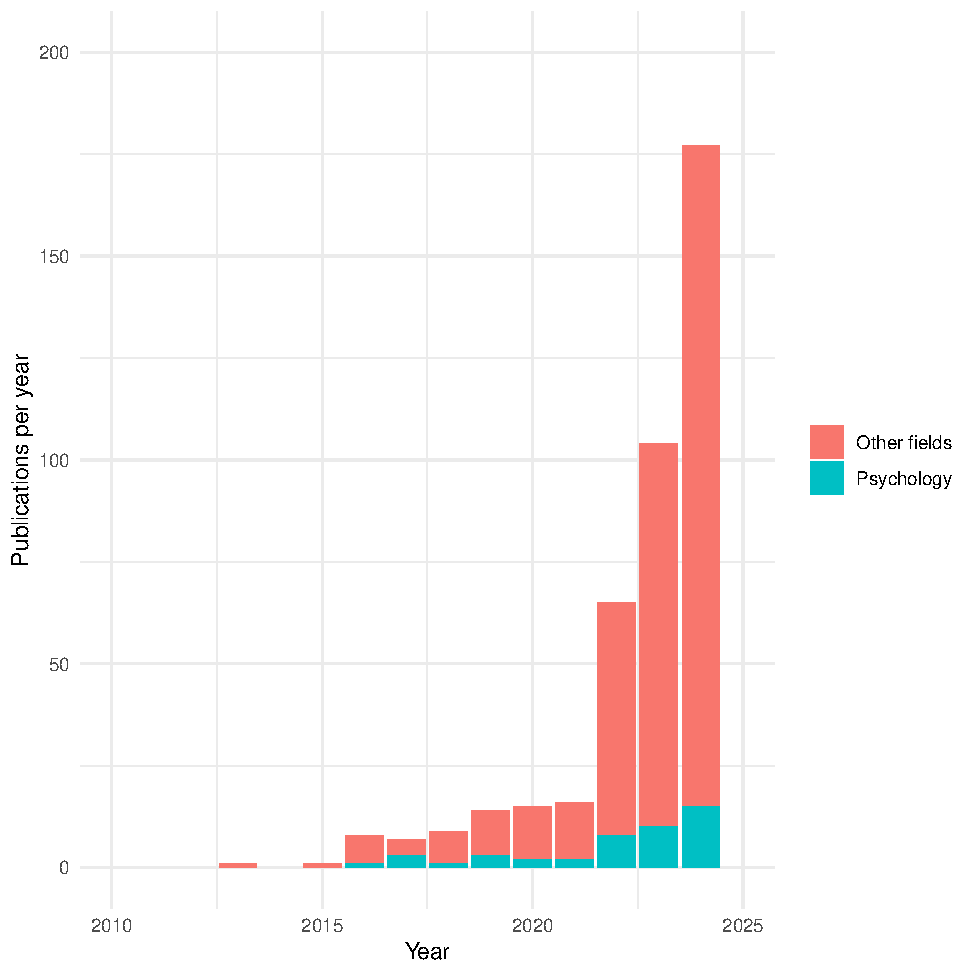
\includegraphics[keepaspectratio]{nca_paper_files/figure-pdf/fig-bib-1.pdf}}

}

\end{figure}%

The appeal of NCA lies in the fact that its logic is not merely
semantic. The method operationalizes necessity in a clear geometric way.
If low values of a condition \(X\) are incompatible with high values of
an outcome \(Y\), then the upper-left corner of the \(X\)-\(Y\)
scatterplot should be empty or nearly empty. NCA quantifies that empty
region, estimates a ceiling line, and translates the geometry of the
scatterplot into an effect size and a bottleneck table. This is
methodologically elegant. It also makes the method highly intuitive: a
predictor is considered important not because the mean of \(Y\) rises
with \(X\), but because the absence or low level of \(X\) places a hard
limit on how high \(Y\) can become
(\citeproc{ref-dulNecessaryConditionAnalysis2016}{Dul, 2016};
\citeproc{ref-dulNecessaryConditionAnalysis2023}{Dul et al., 2023}).

Yet the very features that make NCA attractive also raise a serious
question for psychology. Psychological theories are usually stated in
terms of \emph{latent constructs}, whereas NCA is typically applied to
\emph{observed scores}. Even when researchers use the language of
``intelligence,'' ``motivation,'' ``emotion regulation,'' or
``self-control,'' the empirical input into NCA is generally not the
construct itself, but a scale score, composite, factor score, or
model-based proxy derived from a particular instrument. This is not a
small technical detail. It creates a possible mismatch between the
theoretical object of interest and the empirical object to which NCA is
actually applied. NCA's own guidelines appropriately emphasize the need
for theoretical justification and ``meaningful data,'' and they
explicitly note that the method can be used with indicator scores,
construct or latent-variable scores, and factor scores so long as these
are valid and reliable
(\citeproc{ref-dulNecessaryConditionAnalysis2016}{Dul, 2016};
\citeproc{ref-dulNecessaryConditionAnalysis2023}{Dul et al., 2023};
\citeproc{ref-marchettiNecessityCausalityMental2026}{Marchetti et al.,
2026}). However, once the problem is framed in psychometric terms, the
requirement of ``meaningful data'' becomes much more demanding than it
first appears.

The issue is not simply whether a score is ``good enough'' in the
generic sense of having acceptable reliability. The deeper question is
what it would mean for a necessity claim to be interpretable when the
variables have no natural metric, are measured through ordinal item
responses, depend on identification constraints or score-construction
rules, and may or may not be comparable across groups, instruments, or
studies. In many psychological applications, the substantive conclusion
eventually drawn from NCA is a statement about a \emph{construct}---for
example, that a certain level of intelligence is necessary for
creativity
(\citeproc{ref-karwowskiIntelligenceChildhoodCreative2017}{Karwowski et
al., 2017}). But the quantity to which the method has actually been
applied may be a raw total score, an average of Likert items, a
standardized composite, a factor score estimate, or a latent score
produced by a particular model. Whether these different representations
are interchangeable is itself a psychometric question, not something NCA
settles by construction
(\citeproc{ref-mcneishPsychometricPropertiesSum2023}{McNeish, 2023};
\citeproc{ref-mcneishThinkingTwiceSum2020}{McNeish \& Wolf, 2020};
\citeproc{ref-widamanThinkingThriceSum2022}{Widaman \& Revelle, 2022}).

We argue that the interpretability of NCA becomes especially fragile in
psychology because the method is applied to score geometry while
psychological theories are usually about latent constructs and their
relationships. Once this distinction is taken seriously, several
concerns follow immediately: first, the ``necessary condition'' may be a
property of a score rather than of a construct; second, the estimated
threshold may depend on scale definition and sample range; third,
because NCA relies on the boundary of the data cloud rather than on its
center, the method may be unusually vulnerable to skewness, range
restriction, and measurement error in the parts of the scale that matter
most for the analysis; and fourth, comparability across groups or
instruments may be compromised by measurement noninvariance. Finally,
NCA may not be suited to unveil the \emph{true} data generating process,
which is presumably the main aim of psychological science
(\citeproc{ref-sorjonenNecessityFunctionSkewness2017}{Sorjonen et al.,
2017};
\citeproc{ref-sorjonenPredictingSignificanceNecessity2019}{Sorjonen \&
Melin, 2019}).

\section{What NCA Estimates,
Statistically}\label{what-nca-estimates-statistically}

NCA is not intended to estimate average relations, conditional means, or
structural coefficients. It is a method for identifying whether a
condition constrains an outcome in the sense that certain outcome levels
are impossible when the condition is too low. NCA focuses on
bottlenecks, constraints, and prerequisites. A necessary condition is
therefore not something that \emph{produces} the outcome in the usual
additive sense, but something without which the outcome cannot occur.
Unlike regression or structural equation modeling, which are based on
additive average-effect logic, NCA aims to clarify whether an outcome
does not appear if a specific condition is not given
(\citeproc{ref-dulNecessaryConditionAnalysis2016}{Dul, 2016}).

Operationally, NCA examines the geometry of an \(X\)-\(Y\) scatterplot
(see Figure~\ref{fig-nca}). The central empirical signature of necessity
is an empty or nearly empty upper-left corner, reflecting the absence of
cases with low \(X\) and high \(Y\). This empty area is separated from
the area containing observations by a ceiling line. In the original
formulation, the effect size of a necessary condition is defined as the
ratio of the size of the ceiling zone to the size of the total area in
which observations could occur, that is,

\[
 d = C/S,
\]

where \(C\) is the ceiling zone and \(S\) is the scope. The scope itself
is defined by the minimum and maximum values of \(X\) and \(Y\), either
theoretically or empirically, so that
\(S = (X_{\max}-X_{\min})(Y_{\max}-Y_{\min})\). In other words, the NCA
effect size is literally the proportion of the available data space that
lies above the ceiling line. The larger this empty region is relative to
the scope, the stronger the estimated necessity effect
(\citeproc{ref-dulNecessaryConditionAnalysis2016}{Dul, 2016}).

\begin{figure}

\caption{\label{fig-nca}Example of an NCA plot. The scatterplot shows
the relation between X and Y. NCA evaluates whether X is necessary for Y
by identifying an empty upper-left region, meaning that high values of Y
are absent when X is low. The ceiling lines (CE-FDH and CR-FDH) mark the
estimated boundary of this empty space, while the OLS line is included
only to contrast NCA with standard regression approaches.}

\centering{

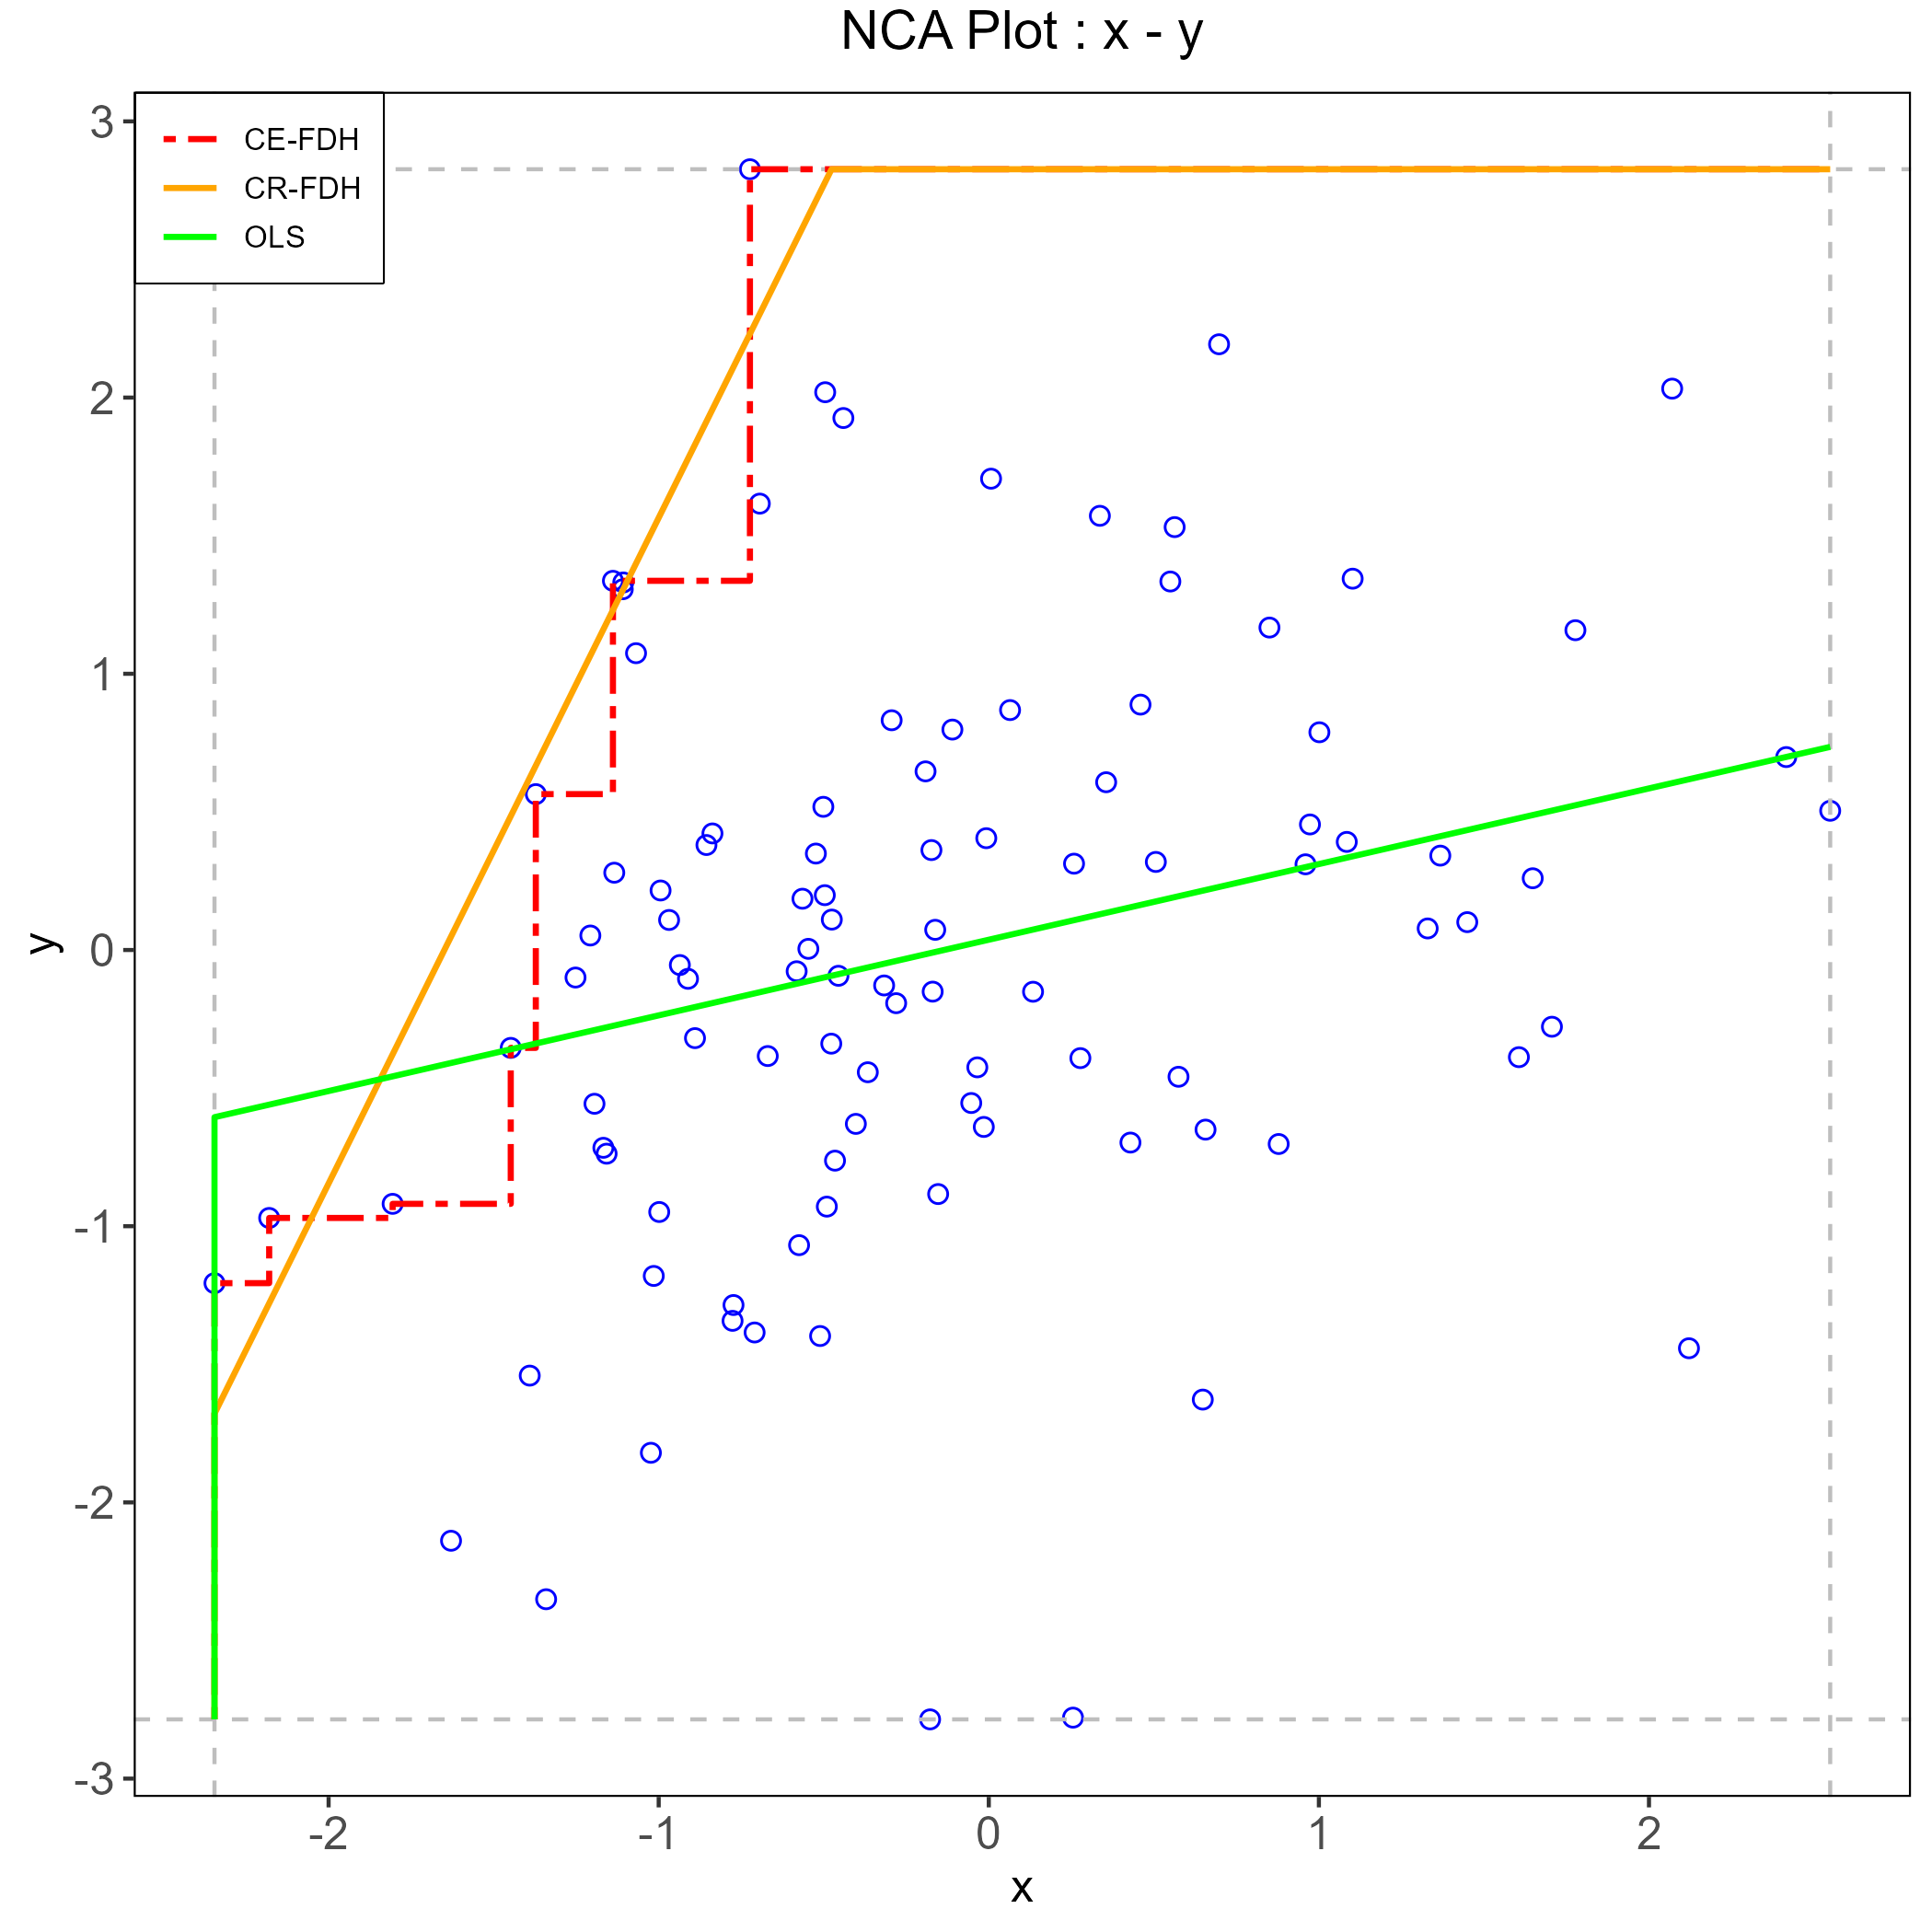
\includegraphics[width=7in,height=\textheight,keepaspectratio]{ncaplot.png}

}

\end{figure}%

This definition has several immediate implications. First, NCA is
explicitly a \emph{boundary} method. It is driven by the contour of the
data cloud, not by its central tendency. Second, the method depends on
the representation of the variables in the observed coordinate system,
because both the ceiling zone and the scope are defined in that system.
Third, unlike a symmetric association measure such as correlation,
necessity is directional: ``\(X\) is necessary for \(Y\)'' is not
equivalent to ``\(Y\) is necessary for \(X\).'' These properties matter
enormously for psychological applications, because they imply that
observed scale definition enters directly into the quantity being
estimated (\citeproc{ref-sorjonenNecessityFunctionSkewness2017}{Sorjonen
et al., 2017}).

To estimate the necessary conditions several ceiling techniques were
proposed, among which CE-FDH and CR-FDH became the default nonparametric
and parametric approaches, respectively. The same article also suggested
generic benchmarks for effect sizes, with values below .10 described as
small, values from .10 to .30 as medium, values from .30 to .50 as
large, and values above .50 as very large. Importantly, for a straight
ceiling line the theoretical maximum effect size is .50; larger values
are expected only when the ceiling is nonlinear. These conventions are
now often reproduced in applied work and shape researchers' judgments
about whether a necessity effect is substantively important
(\citeproc{ref-dulNecessaryConditionAnalysis2016}{Dul, 2016};
\citeproc{ref-dulNecessaryConditionAnalysis2019}{Dul et al., 2019};
\citeproc{ref-marchettiNecessityCausalityMental2026}{Marchetti et al.,
2026}).

NCA's practical output extends beyond a single effect size. The method
also produces \emph{bottleneck tables} that indicate the level of a
condition required to make a given outcome level possible. These
bottleneck levels can be expressed as percentages of the observed range,
as actual values, as percentiles, or as percentages of the maximum. In
applications, these tables are often the most compelling part of the
analysis because they seem to provide directly interpretable thresholds.
Yet the review article explicitly notes that the default bottleneck
table expresses both \(X\) and \(Y\) in percentages of their respective
ranges, with 0\% corresponding to the minimum and 100\% to the maximum.
Thus, the familiar ``minimum required level'' reported by NCA is not a
threshold in an abstract construct space; it is a threshold defined
relative to a particular representation of the observed range
(\citeproc{ref-dulNecessaryConditionAnalysis2023}{Dul et al., 2023}).

NCA has also developed inferential tools
(\citeproc{ref-dulStatisticalSignificanceTest2020}{Dul et al., 2020}).
The statistical significance paper proposes an approximate permutation
test as a minimum statistical test for NCA and recommends that a
condition be treated as necessary only if three requirements are met:
theoretical justification, an effect size greater than zero, and a small
\(p\)-value. The same article also explicitly notes that future
development of NCA could include approaches that model measurement
error, among other extensions. This acknowledgment is especially
relevant for psychology, because it means that even within the NCA
literature the current inferential machinery is not presented as fully
resolving the problem of noisy measurement
(\citeproc{ref-dulStatisticalSignificanceTest2020}{Dul et al., 2020}),
but it also indirectly implies that NCA aims to work with latent
variables and constructs.

Indeed, the crucial point, then, is that NCA estimates a property of the
\emph{observed score space}: the size of a ceiling zone relative to a
scope, plus the associated bottleneck levels implied by the estimated
ceiling line. This make the interpretive leap from ``observed score
bottleneck'' to ``latent psychological necessity'' much larger than it
is often presented to be.

\section{Why Psychological Data Are a Special
Problem}\label{why-psychological-data-are-a-special-problem}

The basic machinery of NCA can be described without reference to any
particular discipline. In principle, the same logic can be applied to
natural metrics such as years of experience, physiological indicators,
or financial resources, as well as to psychometric scores. But
psychological data are not merely another instance of the general case.
They raise special difficulties because the substantive entities of
interest are usually latent constructs, whereas the data available for
analysis are instrument-dependent observations. This distinction affects
not only estimation, but interpretation. A necessity claim is
substantively strong: it implies that an outcome level is impossible
unless a condition reaches at least a certain level. In psychological
research, however, both the condition and the outcome are commonly
measured in ways that are model dependent, scale dependent, and
potentially noncomparable across contexts. For that reason, the move
from NCA's geometry to substantive psychological inference requires much
more justification than is typically acknowledged
(\citeproc{ref-merkleIdentificationScalingLatent2026}{Merkle et al.,
2026}), unless one is interested in the scale-specific values without
any interest in generalizing to (nor informing) substantive theories or
other measurement tools.

\subsection{Constructs Are Latent, but NCA Is Usually Run on Observed
Scores}\label{constructs-are-latent-but-nca-is-usually-run-on-observed-scores}

A first problem is ontological and psychometric at the same time.
Psychological constructs such as intelligence, depression,
self-efficacy, or conscientiousness are generally treated as latent
variables or latent attributes, not as directly observed quantities.
Even when researchers use a composite score in practice, the theoretical
entity to which they wish to generalize is usually not the sum or mean
of the item responses as such, but the underlying construct those items
are intended to represent.

This point matters for NCA because the method nearly always takes
\emph{scores} as its inputs. Those scores may be simple sums, means,
standardized composites, factor scores, or latent-variable estimates
exported from a separate model. NCA does not itself adjudicate the
psychometric adequacy of these inputs. NCA proponents suggest that it
works on any possible measures provided the scores are valid and
reliable. That flexibility is useful from an applied perspective, but it
also means that NCA inherits the unresolved psychometric assumptions of
whatever score-construction method was used upstream
(\citeproc{ref-dulNecessaryConditionAnalysis2023}{Dul et al., 2023}).

For psychology, this is not a marginal concern because score
construction is not a neutral preprocessing step. Sum scoring is itself
a constrained latent-variable model rather than a model-free arithmetic
operation (\citeproc{ref-mcneishThinkingTwiceSum2020}{McNeish \& Wolf,
2020}). Unjustified sum scoring can affect validity, reliability, and
classification based on score cutoffs. This argument does not imply that
sum scores are never acceptable. It does imply, however, that a score
used in downstream analysis embodies assumptions about item equivalence,
weighting, and measurement structure. If those assumptions are weakly
justified, any claim that depends critically on the exact geometry of
the resulting score distribution must be interpreted with caution
(\citeproc{ref-mcneishThinkingTwiceSum2020}{McNeish \& Wolf, 2020}).

A further example comes from McNeish's simulation study showing that the
psychometric properties of sum scores and factor scores can differ even
when the correlation between them is .96 or .98. In his simulations,
factor scores had higher correlations with true scores, greater
sensitivity, and higher reliability than sum scores, despite the very
high correlation between the two score types
(\citeproc{ref-mcneishPsychometricPropertiesSum2023}{McNeish, 2023}).

For NCA, this has an immediate implication. A necessity claim based on a
sum score is not automatically equivalent to a necessity claim about the
corresponding factor score, let alone about the latent construct itself.
If different admissible score representations of the same construct
yield different scatterplot geometries, different ceiling lines, or
different bottleneck thresholds, then the estimated ``necessary
condition'' is partly a function of score construction. In such
circumstances, the strong substantive interpretation---``construct \(X\)
is necessary for construct \(Y\)''---moves beyond what the analysis
itself directly establishes. At minimum, one would need to show that the
NCA result is robust across defensible score representations before
elevating it from a property of the score to a property of the
construct.

\subsection{Thresholds Are
Scale-Dependent}\label{thresholds-are-scale-dependent}

A second problem follows from the fact that NCA thresholds are defined
in the metric of the score representation. In psychometrics, however,
scale is not a transparent mirror of the construct. For latent
variables, scale is established by identification constraints and
parameterization choices. Merkle, Winter, and Fitzsimmons show this very
clearly in the context of ordinal factor analysis. They note that social
scientists often treat ordinal items as though they were continuous, and
they develop ``integer constraints'' that place latent variables on the
scale of the observed, integer-coded ordinal variables
(\citeproc{ref-merkleIdentificationScalingLatent2026}{Merkle et al.,
2026}).

This matters enormously for NCA because the method's effect size and
bottleneck thresholds are defined in terms of the observed coordinate
system. In the original article, the scope is computed from the minima
and maxima of \(X\) and \(Y\), and the effect size is the proportion of
that scope lying above the ceiling line. Bottleneck levels are described
as percentages of the observed range by default, though they may also be
expressed in actual values or percentiles. Consequently, the threshold
NCA reports is inseparable from the representation of the variable on
the score axis. Change the coding of the items, the range of the scale,
the transformation applied to the score, or the model used to produce
latent estimates, and the threshold may change as well, even if the
substantive relationship between the constructs has not.

This is a stronger problem for NCA than for many conventional analyses.
In a regression model, linear rescaling of a predictor changes the
regression coefficient but not the underlying fitted relation in any
substantive sense. With NCA, rescaling or redefining the score affects
not only the numeric threshold reported in the bottleneck table but also
the very quantity used to define effect size, because the scope is part
of the denominator of \(d = C/S\). Even when the form of the ceiling
line is preserved geometrically, the substantive meaning of a bottleneck
expressed as ``55\% of the predictor range'' depends on how that range
itself has been defined. If the observed range is sample dependent or
instrument dependent, so too is the bottleneck.

In psychology, the absence of a natural metric makes this especially
problematic. A score of 3.8 on a five-point Likert average, a factor
score of 0.7 in a standardized latent metric, and an IRT-based score
centered at zero are not simply different labels for the same quantity.
They are different representations whose relation to the underlying
construct depends on model assumptions, item properties, and scaling
choices. Accordingly, when a psychological NCA paper states that ``a
minimum of X is required for Y,'' the statement should not be read as a
scale-free fact about the construct unless the score metric itself has
been justified as substantively interpretable. In many applied settings,
the more defensible reading is narrower: ``within this sample, on this
instrument, under this score-construction rule, the observed score space
exhibits a ceiling pattern consistent with a bottleneck.'' That may
still be of descriptive interest. But it is a substantially weaker claim
than the construct-level interpretation that often appears in the
discussion sections of applied studies (e.g.
\citeproc{ref-urbanWeNeedMetacognition2025}{Urban \& Urban, 2025}).

\subsection{Comparability Across Groups and Instruments Is Not
Guaranteed}\label{comparability-across-groups-and-instruments-is-not-guaranteed}

A third problem concerns comparability. Many psychological questions are
implicitly or explicitly comparative: researchers want to make
statements that generalize across age groups, genders, cultures,
clinical versus nonclinical samples, longitudinal waves, or alternative
instruments purportedly measuring the same construct. Yet such
comparisons are warranted only if the measurement structure is
sufficiently invariant. With ordinal data, this problem is particularly
delicate (\citeproc{ref-dursoScaleLengthDoes2022}{D'Urso et al., 2022}).

This has direct implications for NCA. Suppose an NCA threshold for
``self-control'' is estimated in one group and then rhetorically
generalized to another. If the score does not have the same meaning
across those groups, then the threshold is not comparable in the first
place. The same applies when different instruments are used across
studies. An observed score threshold on one inventory is not
automatically transportable to another inventory, even if both are
intended to measure the same construct. The NCA recommendation
(\citeproc{ref-dulNecessaryConditionAnalysis2023}{Dul et al., 2023}) to
use valid and reliable scores is therefore necessary but insufficient
for psychology. Validity and reliability do not by themselves guarantee
cross-group or cross-instrument comparability (e.g.,
\citeproc{ref-dursoScaleLengthDoes2022}{D'Urso et al., 2022}).

The issue is even broader than formal group comparisons. When
researchers use different translations, response formats, item sets, or
score transformations, they are often implicitly changing the metric,
the scope, and possibly the construct representation itself. If NCA is
then used to estimate bottleneck levels, those levels may differ not
because the underlying psychological necessity relation differs, but
because the measurement system differs. Therefore, any necessity claim
meant to travel across populations, settings, or instruments should be
preceded by evidence that the score space being analyzed is sufficiently
comparable for such transportability to be plausible.

\subsection{Sensitivity to Skewness and Distributional
Shape}\label{sensitivity-to-skewness-and-distributional-shape}

Of all the criticisms directed at NCA, the skewness critique is one of
the most consequential for psychology. Sorjonen and colleauges
(\citeproc{ref-sorjonenNecessityFunctionSkewness2017}{2017}) show in a
simulation study that NCA's calculated necessity effect has a negative
association with the skewness of the predictor and a positive
association with the skewness of the outcome. Most importantly, they
conclude that at least some findings obtained with NCA fall within the
range of what can be expected from the skewness of the predictor and the
outcome alone. Their explanation is intuitive: if low values of \(X\)
are common because \(X\) is negatively skewed and high values of \(Y\)
are common because \(Y\) is positively skewed, then the upper-left
corner of the scatterplot can become sparse even when the variables are
unrelated in any substantively necessary sense.

The later paper by Sorjonen and Melin
(\citeproc{ref-sorjonenPredictingSignificanceNecessity2019}{Sorjonen \&
Melin, 2019}) extends the concern to NCA's inferential machinery. They
report that the permutation-based significance test can yield
significant results even when the true population necessity effect is
very weak, and that in some situations the significance of the necessity
effect increases with a greater degree of \emph{sufficiency}, which they
regard as paradoxical for a method aimed at identifying necessary but
not sufficient conditions.

These concerns are particularly important in psychology because
nonnormality is not an exotic edge case
(\citeproc{ref-cainUnivariateMultivariateSkewness2017}{Cain et al.,
2017}; \citeproc{ref-toffaliniClustersThatAre2024}{Toffalini et al.,
2024}). Although NCA does not assumes normality, the kinds of
distributional asymmetries that are routine in psychological data are
exactly the kinds of features that can create or exaggerate the
sparse-corner patterns on which NCA relies
(\citeproc{ref-sorjonenNecessityFunctionSkewness2017}{Sorjonen et al.,
2017};
\citeproc{ref-sorjonenPredictingSignificanceNecessity2019}{Sorjonen \&
Melin, 2019}).

This should change how psychological researchers think about an empty
corner. In a domain with natural metrics and relatively well-behaved
distributions, an empty upper-left region may plausibly reflect a
genuine constraint. In psychology, however, the same geometry may arise
because the predictor is bounded and concentrated at the high end,
because the outcome is bounded and concentrated at the low end, or
because the response categories compress information. None of these
explanations is inconsistent with the NCA pattern as such.

\subsection{Sensitivity to Range Restriction and Sample
Composition}\label{sensitivity-to-range-restriction-and-sample-composition}

Another source of fragility is range restriction. NCA's effect size
depends on the scope, which is defined by the observed or theoretical
minima and maxima of the variables, and its bottleneck tables are often
reported relative to the observed range. This means that the magnitude
of the necessity effect and the associated thresholds are not immune to
the composition of the sample.

In psychology, range restriction is often structural rather than
accidental. Researchers may study high-achieving students, patients
meeting diagnostic cutoffs, individuals selected into treatment, or
convenience samples drawn from university populations. Many
psychological scales also have bounded ranges and exhibit floor or
ceiling effects in ordinary use. Under such conditions, the observed
minima and maxima of the scores do not merely summarize the sample; they
define the coordinate system in which the necessity effect is
calculated. A bottleneck that appears substantial within a restricted
sample may look weaker in a broader sample, and a threshold expressed as
a percentage of range may shift because the empirical range changes, not
because the underlying theory has changed.

Sample composition is also rarely representative because psychological
constructs frequently covary with background characteristics that
influence both score distribution and the likelihood of inclusion in the
sample. For example, age, education, language background, or clinical
severity can affect not only the average level of a measure but also
individuals' propensity in participating in studies. If NCA is applied
without attending to these issues, the estimated bottleneck may partly
reflect who was sampled rather than a general feature of the construct
relation.

\subsection{Sensitivity to Measurement Error Near the
Boundary}\label{sensitivity-to-measurement-error-near-the-boundary}

An additional source of fragility concerns measurement error. NCA is a
boundary method, so its inferential weight is concentrated on a
relatively small number of cases lying near the ceiling. Errors
affecting those cases can have disproportionate consequences for the
location of the ceiling line, the size of the empty corner, and the
resulting bottleneck values. Dul and colleagues
(\citeproc{ref-dulStatisticalSignificanceTest2020}{2020}), however,
explicitly recognize that NCA methods do not handle measurement error to
date.

In psychological measurement error is intrinsic to the process of using
item responses to infer latent standing. Moreover, the precision of
psychological scores often varies across the score distribution. McNeish
and Dumas
(\citeproc{ref-mcneishReliabilityRepresentativenessHow2025}{2025}) note
that reliability can be conditional, such that scores in certain parts
of the distribution are more reliable than others. This observation is
especially relevant for NCA because the method effectively asks the
analyst to pay special attention to certain parts of the range, namely,
those close to the boundary that determine whether high \(Y\) is
compatible with low \(X\).

The implications are straightforward. If scores near the relevant
ceiling region are measured less precisely than scores elsewhere, then
the geometric pattern that NCA interprets as evidence of a bottleneck
may partly be a by-product of differential precision. Likewise, if a few
cases appear in the ostensibly empty upper-left corner because of
response noise, careless responding, or unstable measurement at the
extremes, the analyst faces a difficult interpretive choice: treat them
as substantive falsifications of necessity, or treat them as measurement
artifacts (\citeproc{ref-dulNecessaryConditionAnalysis2016}{Dul, 2016}).
The original NCA framework acknowledges the possibility of outliers and
even discusses ``virtually necessary'' conditions in stochastic terms.
But in psychological data, the outlier-versus-error distinction is often
not adjudicable from the score data alone.

\section{Simulation Study}\label{simulation-study}

The preceding arguments imply that NCA results could vary depending on
basic psychometric issues. In psychological research, however, a method
requires that the estimated effects remains fairly stable when
psychometric features of the observed scores are changed. To prove the
points raised, we conducted a simulation study varying multiple features
of psychological measurement, including score construction, loading
strength and reliability, response formats, threshold placement, and
sample restriction. Additionally, we estimated the robustness of the
results across multiple sample sizes and latent association values.

\subsection{Simulation design}\label{simulation-design}

Each replication followed the same sequence. First, we generated one
latent paired dataset for a predictor construct \(X\) and an outcome
construct \(Y\). Second, we estimated a latent-reference NCA effect on
those latent variables. Third, starting from that same latent dataset,
we generated multiple observed versions of the variables by altering one
psychometric feature at a time. Fourth, we re-estimated NCA on each
observed-score dataset. Because all observed conditions within a
replication were derived from the same latent source, differences among
conditions can be directly attributed to the measurement or sampling
manipulation rather than to differences in the underlying latent
relation.

\subsection{Latent data-generating
model}\label{latent-data-generating-model}

For each replication, latent data were generated from a simple linear
model. A latent predictor \(\eta_X\) was sampled from a standard normal
source and standardized within replication. A latent outcome \(\eta_Y\)
was then generated as \(\eta_Y = \beta_\eta X + \epsilon\), where
\(\beta\) controlled the strength of the latent association and the
residual variance was chosen so that the population variance of
\(\eta_Y\) was approximately one. This specification does not impose a
latent necessity structure \footnote{Necessity structures spuriously
  `emerge' when analyzing correlated data
  (\citeproc{ref-sorjonenQuestionableNecessityEffects2026}{Sorjonen et
  al., 2026}).}. Instead, it creates a stable latent relation and then
asks how NCA behaves when the observed-score representation of that
relation is altered. The latent-level NCA effect can therefore be
interpreted as a benchmark {[}though spurious{]} quantity for each
replication, not as a theoretical ``true necessity'' parameter in a
population model.

Sample size and latent association strength were treated as outer design
factors. The simulation crossed sample sizes of \(n = 250\), \(500\),
and \(1000\) with latent association values of \(\beta = 0.20\),
\(0.40\), and \(0.60\). For each design cell, 1000 replications were
generated. This yielded a broad set of conditions ranging from
relatively weak to moderate latent associations and from common to
comparatively large sample sizes in psychological research.

\subsection{Measurement model and observed-score
construction}\label{measurement-model-and-observed-score-construction}

Observed variables were generated from the latent variables through a
unidimensional ordinal item model. For each construct, six items were
simulated by combining the latent variable with item-specific residual
error, \(y^*_{ij} = \lambda_j \eta_i + e_{ij}\), where \(\lambda_j\)
denotes the item loading and the residual variance was set to
\(1-\lambda_j^2\). The continuous response propensities \(y^*_{ij}\)
were then discretized into ordinal response categories using fixed
thresholds. Unless otherwise manipulated, the baseline measurement setup
used six items per scale, loadings of \(\lambda = 0.70\), and five
response categories.

Thresholds were constructed to yield a psychologically plausible
response format in which middle categories were more common than extreme
categories. Observed scale scores were then formed from the item
responses. Sum scores were used as the default representation throughout
the simulation, and factor scores were included only in the
score-construction block as an alternative scoring method. Factor scores
were obtained from separate one-factor confirmatory factor analyses for
the \(X\) and \(Y\) item sets, estimated with an ordinal-data CFA model
using WLSMV.

\subsection{Experimental blocks}\label{experimental-blocks}

All manipulations were implemented one factor at a time, with the
remaining psychometric features held at their baseline values. This made
it possible to isolate how much each feature altered the NCA estimate
relative to the latent-reference effect.

\subsubsection{Score construction}\label{score-construction}

The first block examined whether the estimated NCA effect depends on how
the same observed item responses are converted into scale scores. Using
the same item-level data, we computed both sum scores and model-based
factor scores and applied NCA to each representation. This block
therefore isolates score-construction dependence while holding the
latent data, item parameters, and ordinal responses fixed.

\subsubsection{Reliability and loading
strength}\label{reliability-and-loading-strength}

The second block varied loading strength to assess the role of
measurement quality. Loadings were set to \(\lambda = 0.50\), \(0.70\),
and \(0.85\), representing comparatively weak, moderate, and strong
measurement. All other aspects of the measurement model were held
constant, and observed variables were formed as sum scores. Because
lower loadings increase the amount of item-specific noise in the
observed scores, this block evaluates whether measurement error alters
the empty-corner geometry on which NCA relies.

\subsubsection{Number of response
categories}\label{number-of-response-categories}

The third block varied the number of ordinal response categories while
holding the latent relation and baseline loading structure constant. We
compared scales with 4, 5, and 7 response options. If NCA estimates
depend on whether the construct is measured with four, five, or seven
categories, keeping all other measurement properties fixed, then the
resulting necessity claim becomes partly a function of questionnaire
design.

\subsubsection{Threshold placement and induced score
asymmetry}\label{threshold-placement-and-induced-score-asymmetry}

The fourth block examined the effect of threshold placement. Here the
number of response categories was held constant and the full set of
thresholds was shifted upward or downward, thereby changing how easily
low, middle, and high observed responses were endorsed. We calibrated
three levels of threshold severity so that, under the baseline
measurement setup, the resulting sum scores exhibited approximately
mild, moderate, and strong asymmetry, targeting observed skewness values
around 0.25, 0.40, and 0.60. Both lower and upper shifts were examined,
so that asymmetry could be induced in either direction.

Item wording, endorsement difficulty, and response-style effects can all
change where thresholds fall, even when the underlying latent relation
remains the same. Accordingly, we do not treat skewness as a
latent-distribution manipulation. Instead, we evaluate whether NCA
changes when asymmetry is introduced through the measurement layer
itself.

\subsubsection{Range restriction and sample
composition}\label{range-restriction-and-sample-composition}

The fifth block addressed range restriction. Starting from the same
latent dataset, we selected subsamples by restricting either the latent
predictor or the latent outcome to lower- or upper-range segments.
Operationally, restrictions were implemented on the latent variables
using percentile cutoffs that retained approximately 70\% of cases in
each selected sample. We considered four restriction conditions:
lower-range and upper-range restriction on \(\eta_X\), and lower-range
and upper-range restriction on \(\eta_Y\).

This decomposition makes it possible to separate changes due to sample
selection from additional changes introduced by measurement and scoring
after selection.

\subsection{NCA estimation and evaluation
criteria}\label{nca-estimation-and-evaluation-criteria}

All NCA estimates were computed with a single ceiling technique, the
nonparametric CE-FDH method. We selected this estimate as it is the most
widely used and its use is suggested for psychological data
(\citeproc{ref-dulNecessaryConditionAnalysis2016}{Dul, 2016};
\citeproc{ref-dulNecessaryConditionAnalysis2023}{Dul et al., 2023};
\citeproc{ref-marchettiNecessityCausalityMental2026}{Marchetti et al.,
2026}). The primary outcome considered was the NCA effect size \(d\),
defined as the proportion of the observed scope occupied by the ceiling
zone. In addition, the simulation stored auxiliary NCA outputs such as
bottleneck information, together with descriptive properties of the
analyzed \(X\) and \(Y\) distributions, including their means, standard
deviations, skewness, and kurtosis.

For each observed condition, we also retained the difference between the
observed effect and the latent full-sample reference. For
range-restriction conditions, we also retained differences from the
condition-specific latent restricted-sample reference.

Because the primary question concerned interpretability and stability
rather than inferential rejection we did not conduct nor reported any
permutation-based significance testing.

All results are available on the GitHub page of the project and in the
supplementary materials. Here we will focus on the stability of the
effect sizes only.

\subsection{A critical caveat}\label{a-critical-caveat}

A careful reader probably recognized an issue in our simulation
approach: We did not simulate any necessity scenario. Our
data-generating process does not imply the existence of any necessary
condition in the observed data but only latent associations between the
data. As a consequence, any presence of a necessity effect is by
definition a false positive. However, NCA always detects some degree of
necessity conditions when two variables are correlated
(\citeproc{ref-sorjonenQuestionableNecessityEffects2026}{Sorjonen et
al., 2026}), but the proponents of NCA in psychology suggested using
this method at least as an accompanying descriptive tool that integrates
`classical' association-based studies. For instance, about the use of
archival data, Marchetti and colleagues state ``\emph{Re-analyzing these
data with a different causal perspective can result in new complementary
insights}''
(\citeproc{ref-marchettiNecessityCausalityMental2026}{Marchetti et al.,
2026}).

With our simulation we show how not even a conservative use of NCA that
does not aim to unveil any \emph{true} underlying necessity is
defensible without strong psychometric assumptions or substantive
robustness tests.

\section{Results}\label{results}

The complete set of results is available in the project repository and
in the supplementary materials. Here we focus on the main descriptive
pattern: how much NCA's effect size \(d\) changes when the latent
relation is held constant but the observed-score representation is
altered. Figure~\ref{fig-summary} reports a compact summary averaged
across sample-size and latent-association conditions.

Across all summarized conditions, the average observed NCA effect ranged
from 0.08 to 0.17, even though the underlying latent relation was fixed
within each block.

\begin{table}

{\caption{{}{\label{tbl-summary}}}
\vspace{-20pt}}

\end{table}

\begin{figure}

\caption{\label{fig-summary}Summary of the simulation results across all
experimental blocks. Points show the average observed NCA effect size
for each condition after averaging across sample size and latent
association (𝛽); vertical intervals indicate uncertainty around these
averages.}

\centering{

\pandocbounded{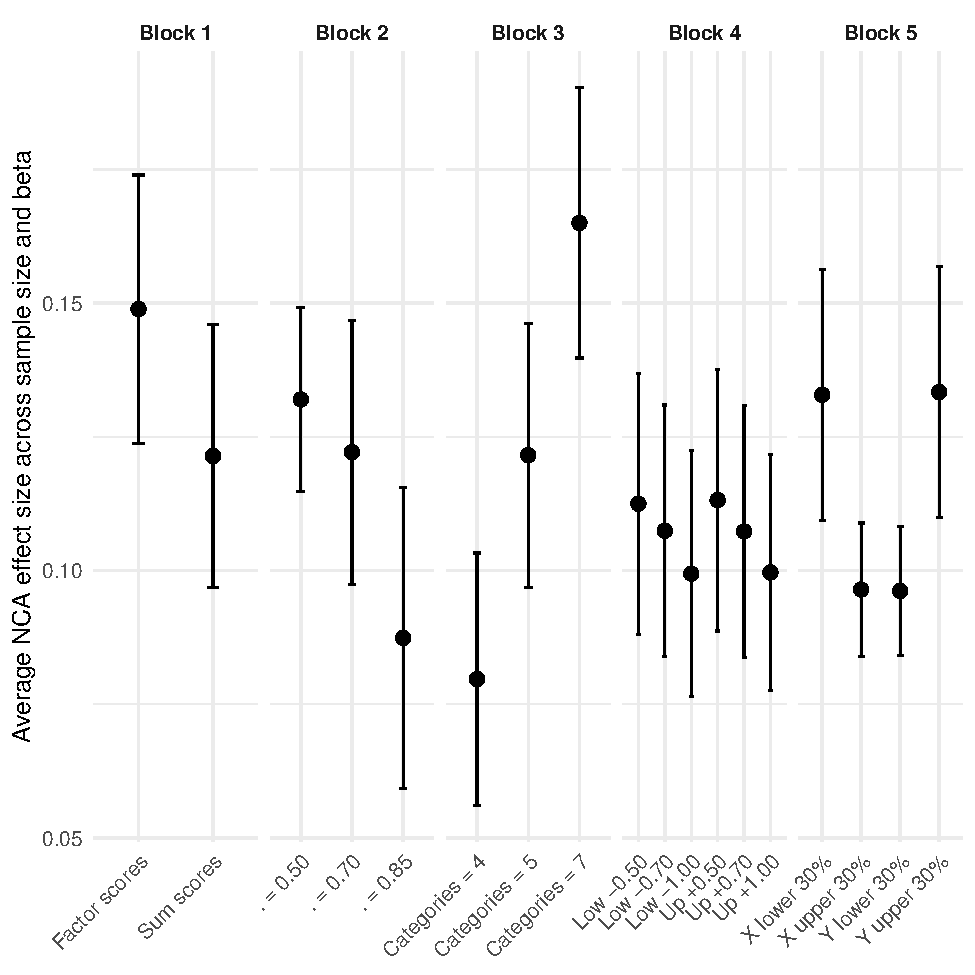
\includegraphics[keepaspectratio]{nca_paper_files/figure-pdf/fig-summary-1.pdf}}

}

\end{figure}%

\subsection{Block 1: Score
construction}\label{block-1-score-construction}

For score construction, factor scores consistently produced larger
effects than sum scores when latent association and sample size were
held constant (see Figure~\ref{fig-block1}). Averaged across design
cells, factor scores yielded \(d =\) compared with \(d =\) for sum
scores, a difference of and a relative increase of about \% over the
sum-score condition. This is a nontrivial shift given that both scores
were computed from the same item responses. In substantive terms, the
apparent strength of the necessity relation depended partly on the
scoring rule rather than only on the latent relation itself.

Figure~\ref{fig-block1} also shows that both score types followed the
same general trend across design cells: effect sizes became smaller when
the latent association was weaker and when sample size was larger.
Still, the factor-score advantage was visible across the design, which
means that a purely psychometric scoring decision was enough to alter
the magnitude of the NCA estimate in a systematic way.

\begin{figure}

\caption{\label{fig-block1}Effects of score construction on observed NCA
estimates.}

\centering{

\pandocbounded{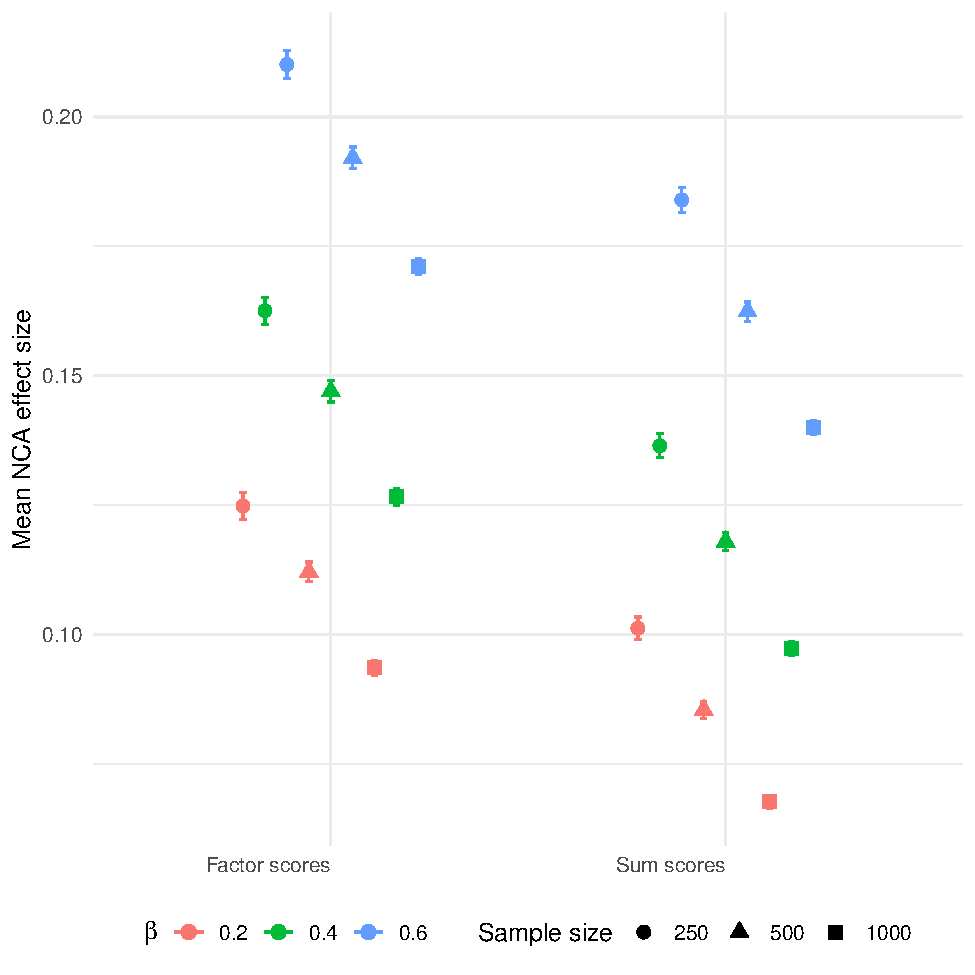
\includegraphics[keepaspectratio]{nca_paper_files/figure-pdf/fig-block1-1.pdf}}

}

\end{figure}%

\subsection{Block 2: Loadings and
reliability}\label{block-2-loadings-and-reliability}

When loading strength was varied, the estimated NCA effect changed in
the opposite direction from what might be expected if stronger
measurement simply sharpened a construct-level necessity relation (see
Figure~\ref{fig-block2}). Averaged across sample sizes and latent
associations, the mean effect was \(d =\) at \(\lambda = 0.50\), \(d =\)
at \(\lambda = 0.70\), and \(d =\) at \(\lambda = 0.85\). The change
from the lowest to the highest loading corresponded to a reduction of in
the average observed effect size (\%).

This pattern indicates that improving the measurement relation between
items and the latent variable did not make the observed NCA effect
converge upward on some stable construct-level quantity. Instead, the
estimated effect shrank as the scale more closely reflected the
underlying latent variable. The cell-level figure showed the same
general dependence on \(\beta\) and sample size observed elsewhere, but
the main result is that reliability itself materially changed the
apparent necessity effect.

\begin{figure}

\caption{\label{fig-block2}Effects of loading strength on observed NCA
estimates}

\centering{

\pandocbounded{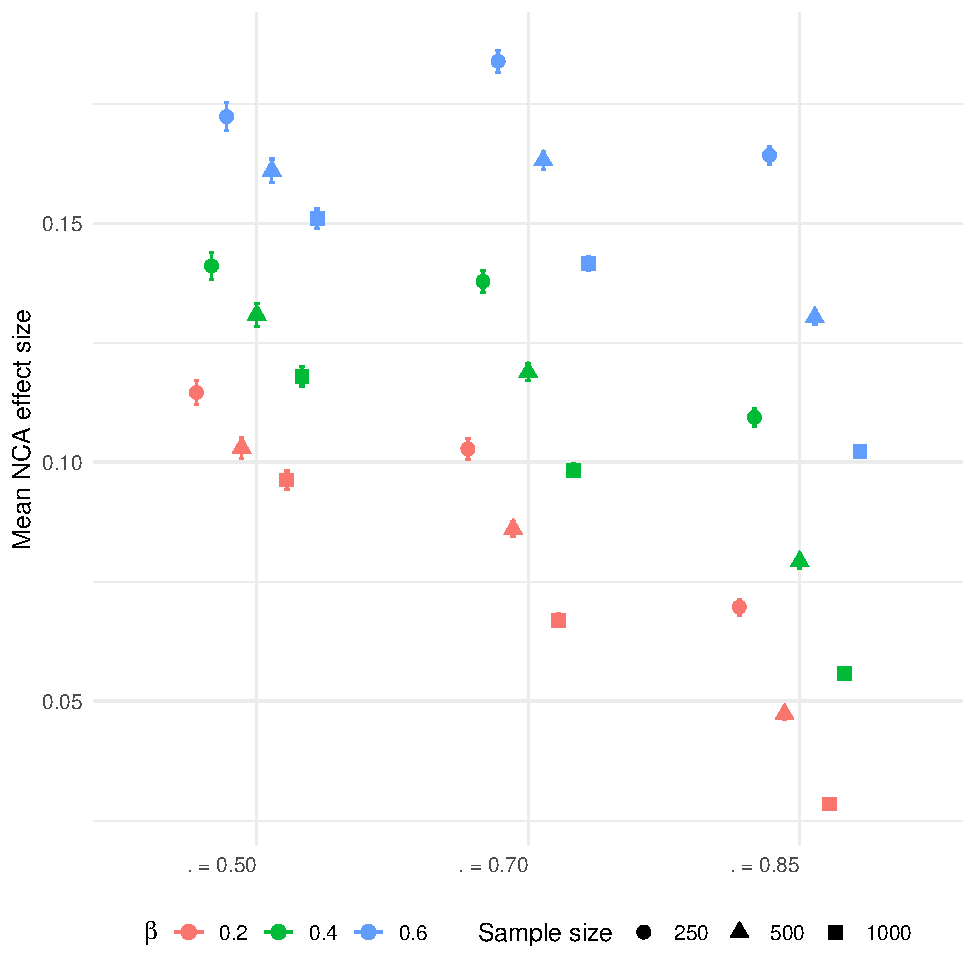
\includegraphics[keepaspectratio]{nca_paper_files/figure-pdf/fig-block2-1.pdf}}

}

\end{figure}%

\subsection{Block 3: Number of response
categories}\label{block-3-number-of-response-categories}

The number of available response categories had one of the largest
effects in the entire simulation (see Figure~\ref{fig-block3}): the
average observed effect was with four categories, with five categories,
and with seven categories. Moving from four to seven categories
therefore increased the average NCA estimate by without any change in
the latent relation.

This result is especially important for psychological research because
the difference between 4-, 5-, and 7-point scales is usually treated as
a routine instrument-design choice rather than as a substantive
theoretical manipulation. Here, however, that routine choice was enough
to move the NCA estimate from a small effect to the upper part of the
medium range, despite no change in the latent relation. As in the
previous blocks, the figures also showed smaller effects at lower
\(\beta\) values and at larger sample sizes.

\begin{figure}

\caption{\label{fig-block3}Effects of the number of response categories
on observed NCA estimates}

\centering{

\pandocbounded{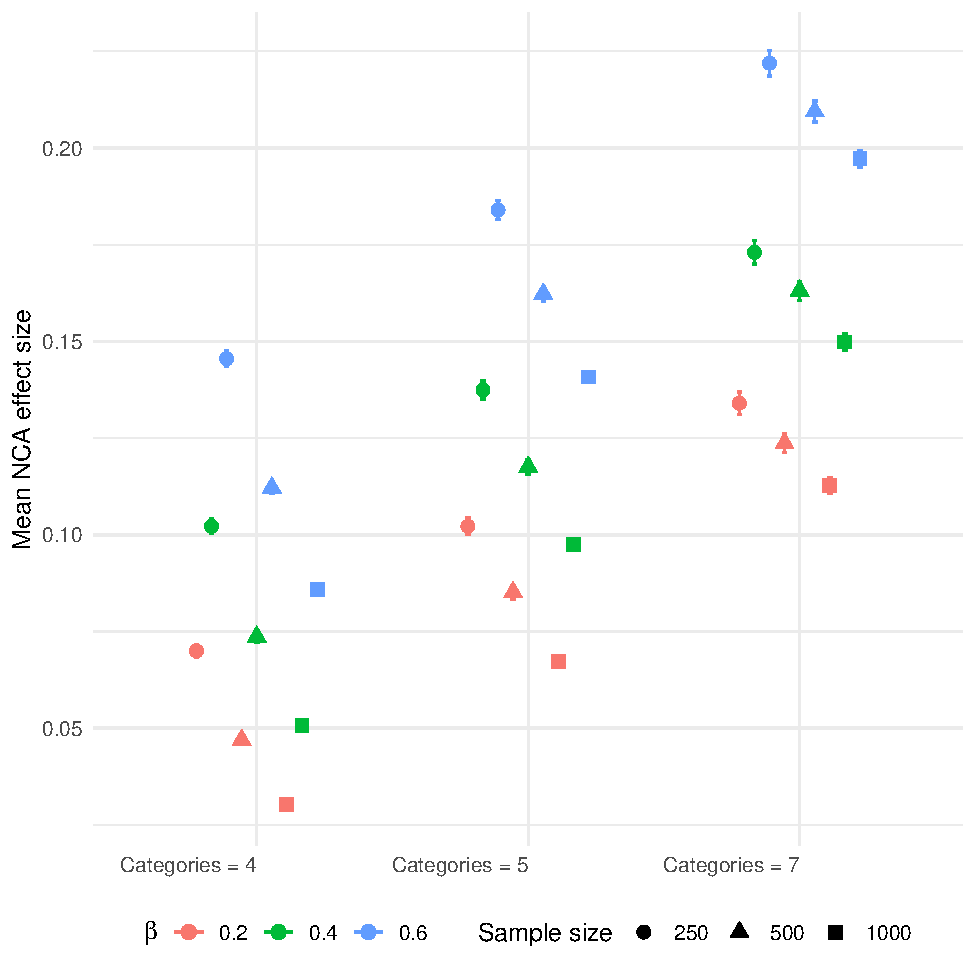
\includegraphics[keepaspectratio]{nca_paper_files/figure-pdf/fig-block3-1.pdf}}

}

\end{figure}%

\subsection{Block 4: Threshold shift}\label{block-4-threshold-shift}

In the fourth block (see Figure~\ref{fig-block4}), response styles were
shifted toward higher or lower categories, thereby inducing the kind of
asymmetry often observed in Likert data. The impact on NCA was more
modest than in some other blocks, but still systematic. For lower
shifts, the mean effect was , , and for magnitudes of 0.50, 0.70, and
1.00, respectively; for upper shifts, the corresponding values were , ,
and . The pattern was nearly symmetric across lower and upper shifts,
with the largest shifts reducing the average observed effect to about
NaN.

Again, smaller latent associations and larger sample sizes were
associated with smaller observed NCA effects.

\begin{figure}

\caption{\label{fig-block4}Effects of threshold shifts on observed NCA
estimates}

\centering{

\pandocbounded{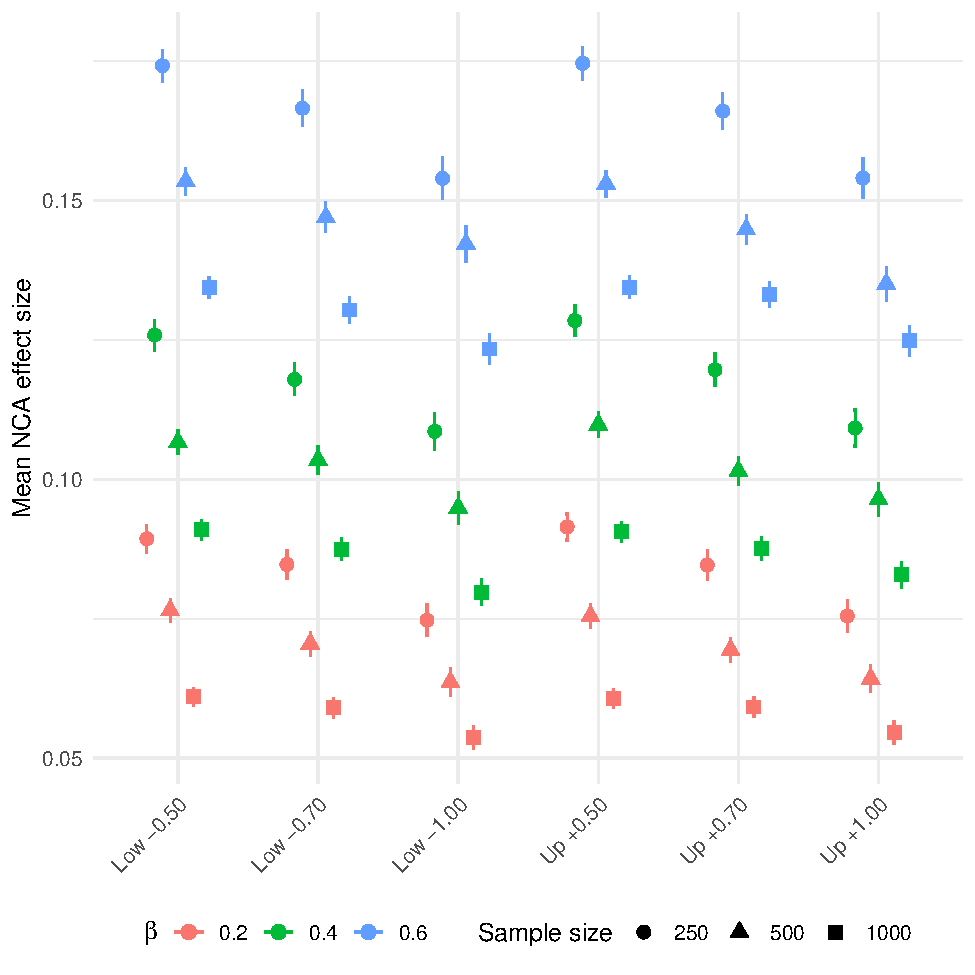
\includegraphics[keepaspectratio]{nca_paper_files/figure-pdf/fig-block4-1.pdf}}

}

\end{figure}%

\subsection{Block 5: Range restriction}\label{block-5-range-restriction}

In the final block (see Figure~\ref{fig-block5}), we induced range
restriction by excluding either the lower or upper 30\% of the
population on \(X\) or \(Y\). This manipulation substantially changed
the observed NCA estimates. Averaged across sample sizes and latent
associations, the mean effect was when the lower 30\% of \(X\) was
excluded, when the upper 30\% of \(X\) was excluded, when the lower 30\%
of \(Y\) was excluded, and when the upper 30\% of \(Y\) was excluded.
The difference between the larger-effect and smaller-effect restriction
conditions was therefore about .

This result shows that the NCA estimate depended not just on whether the
sample was restricted, but on which portion of the latent distribution
was underrepresented. In other words, the method was sensitive to sample
composition in a way that directly affected the apparent size of the
empty corner. For psychological applications, this implies that
necessity claims may partly reflect selection into the sample rather
than a stable feature of the construct relation.

\begin{figure}

\caption{\label{fig-block5}Effects of range restriction on observed NCA
estimates}

\centering{

\pandocbounded{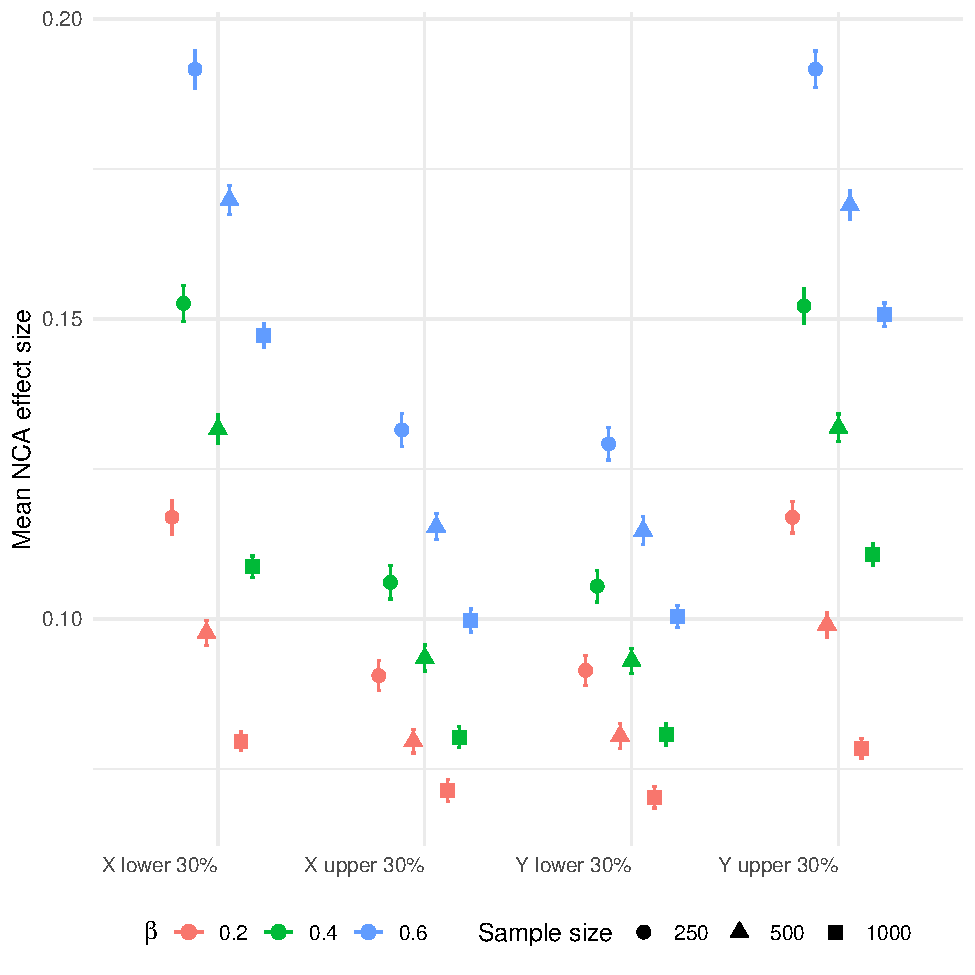
\includegraphics[keepaspectratio]{nca_paper_files/figure-pdf/fig-block5-1.pdf}}

}

\end{figure}%

\subsection{Sample size
considerations}\label{sample-size-considerations}

From the previous simulation a paradoxical problem emerged: the effect
size estimates varied as a function of sample size. We therefore
extended the basic simulation across multiple sample sizes. Using a
fixed \(\beta = 0.40\) latent association and estimating NCA directly on
the latent variables, the mean effect decreased from 0.2 at N = 250 to
0.18 at N = 2000, and it continued to decline up to 0.17 at N = 10000,
even after the curve began to flatten (see Figure~\ref{fig-n}).

This pattern is difficult to reconcile with the idea that \(d\) captures
a stable population feature of a necessity relation. If the underlying
latent relation is held constant and the estimate nonetheless declines
as more data are observed, then the NCA effect cannot be interpreted
straightforwardly as a sample-size-invariant construct property.
Instead, it appears to depend partly on the probability that
increasingly large samples will populate regions of the \(X\)-\(Y\)
space that smaller samples leave empty by chance. That result
strengthens the broader conclusion of the article: in psychological
data, NCA often tracks properties of observed-score geometry rather than
stable properties of latent constructs.

\begin{figure}

\caption{\label{fig-n}Sample-size dependence of the latent-level NCA
effect}

\centering{

\pandocbounded{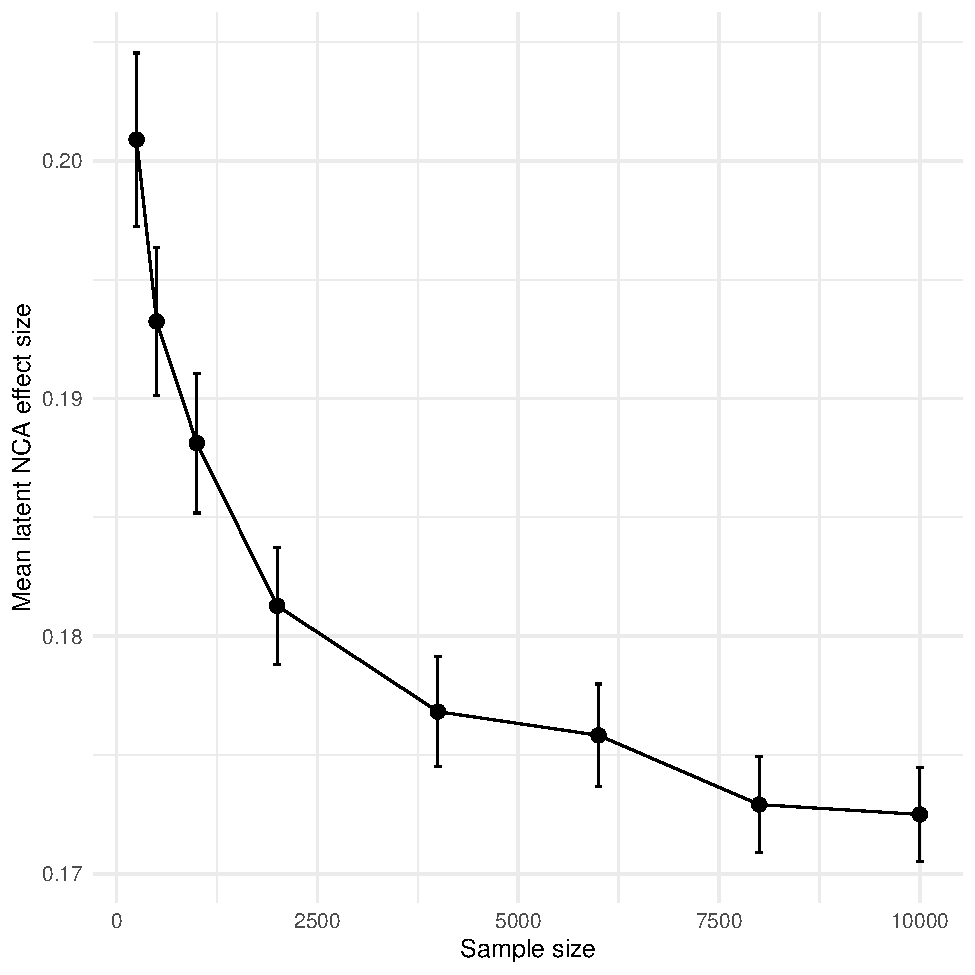
\includegraphics[keepaspectratio]{nca_paper_files/figure-pdf/fig-n-1.pdf}}

}

\end{figure}%

\section{Discussion}\label{discussion}

The present study examined a simple but consequential question for
psychological research: how much can the estimated NCA effect change
solely because the observed variables are scored, discretized, or
sampled differently? Across all simulation blocks, the answer was clear.
The observed NCA effect was not stable. It changed as a function of
score construction, loading strength, number of response categories,
threshold placement, range restriction, and sample size, even though the
underlying latent relation was unchanged within each paired replication.
This is exactly the pattern one would expect if NCA in psychology is
operating primarily on the geometry of observed-score distributions
rather than on a construct-level necessity relation.

The first implication is psychometric. In these simulations, factor
scores yielded systematically larger effects than sum scores, despite
being computed from the same item responses, with mean effects of about
0.15 and 0.12, respectively. Likewise, routine questionnaire design
choices mattered substantially: moving from four to seven response
categories increased the average observed effect from about 0.08 to
0.17, and threshold shifts that induced plausible skewness in either
direction still altered the estimated effect in a systematic way. These
are not exotic manipulations. They are ordinary features of
psychological measurement. If an NCA estimate changes this much when the
scoring rule or response format changes, then the resulting necessity
claim cannot be treated as a stable property of the latent constructs
alone.

The reliability block strengthens that conclusion further. When loadings
increased from .50 to .85, the mean observed effect decreased from about
0.13 to 0.09. In other words, improving the relation between the items
and the latent variable did not make the observed NCA estimate converge
upward on a clearer construct-level quantity. It moved in the opposite
direction. That result is especially problematic for psychological
applications, because it implies that stronger measurement does not
reveal a hidden necessity relation more cleanly. Instead, the observed
necessity effect may partly depend on the distortions introduced by
noisier measurement.

The range-restriction results point to a parallel sampling problem.
Excluding the lower 30\% of the latent predictor or the upper 30\% of
the latent outcome produced average effects of about 0.13, whereas
excluding the upper 30\% of the latent predictor or the lower 30\% of
the latent outcome produced effects closer to 0.10. Thus, NCA was
sensitive not only to whether the sample was restricted, but to which
part of the distribution was missing. In psychological research, where
convenience samples, selective participation, institutional filters, and
attrition are common, this is a serious concern. Apparent bottlenecks
may partly reflect how the sample was composed rather than any stable
necessity structure in the underlying constructs.

The most damaging result, however, may be the sample-size pattern. In
the latent-only extension, with the latent relation fixed at
\(\beta = 0.40\), the mean NCA effect decreased from about 0.20 at
\(N = 250\) to about 0.18 at \(N = 2000\), and then continued to decline
to about 0.17 by \(N = 10000\). That pattern is difficult to reconcile
with the idea that NCA is estimating a stable population feature. If the
data-generating relation is unchanged but the effect shrinks as more
observations are collected, then the estimate is at least partly a
function of finite-sample sparsity. Larger samples are simply more
likely to populate regions of the \(X\)-\(Y\) space that smaller samples
leave empty by chance. Under ordinary stochastic relations, the empty
corner is therefore not strong evidence for an underlying necessity
structure; it is often evidence that the sample has not yet filled the
corner.

This result also clarifies a deeper theoretical issue. The simulations
did not generate any true necessity process. The latent data-generating
model was associational and stochastic, not boundary-based, and the
manuscript explicitly acknowledges that any detected necessity effect is
therefore, in that strict sense, a false positive. That caveat is not
incidental. It reveals that the central question is not merely whether
NCA is statistically sensitive, but whether a necessity model is
theoretically admissible in the first place. A directional or even
causal hypothesis is not enough. Most psychological theories imply that
higher levels of one construct make an outcome more likely, more
intense, or more stable on average. They do not imply that below some
threshold of \(X\), high values of \(Y\) are structurally impossible.
Yet that stronger claim is what a necessity interpretation requires.

For that reason, the common suggestion that NCA can be used as a
conservative add-on to regression or other average-effect models
(\citeproc{ref-dulNecessaryConditionAnalysis2016}{Dul, 2016};
\citeproc{ref-dulNecessaryConditionAnalysis2023}{Dul et al., 2023};
\citeproc{ref-marchettiNecessityCausalityMental2026}{Marchetti et al.,
2026}) is much less convincing and more damaging than it first appears.
When the underlying theory is probabilistic, adding NCA does not reveal
a deeper layer of causal structure. It risks redescribing the same
stochastic relation in stronger language than the theory actually
warrants. In that sense, NCA may be not only uninformative but
counterproductive in psychological research: it can encourage
researchers to speak as if they had identified a prerequisite or
bottleneck when, in fact, they have only detected an observed empty
corner whose size depends on scoring, thresholds, sample composition,
and sample size. The present simulations show that even this
conservative descriptive use is difficult to defend without unusually
strong psychometric justification and extensive robustness checks.

Taken together, these results suggest that the main burden of proof
should be reversed. In psychology, NCA should not be treated as an
attractive supplement that becomes acceptable whenever \(X\) plausibly
predicts \(Y\). Instead, it should be reserved for situations in which
the substantive theory independently implies a genuine boundary-type
process: that is, a process in which some levels of the outcome are
impossible, not merely improbable, below some level of the predictor.
Such cases are likely to be rare. Indeed, many of the clearest
``necessities'' in psychology are not discovered empirical laws at all,
but imposed thresholds, such as diagnostic cut-offs, selection rules, or
administrative criteria. Those boundaries are often created by human
classification decisions rather than uncovered from the latent structure
of psychological constructs.

The practical implication is therefore not simply that researchers
should be more careful when applying NCA. It is that, in most ordinary
psychological applications, the method is unlikely to identify a
construct-level ground truth. At best, it describes constraints in a
particular observed-score space under a particular scoring rule,
response format, and sample composition. At worst, it converts
finite-sample sparsity and measurement artifacts into substantively
inflated claims about necessity. The broader conclusion of the article
is thus not that necessity relations can never exist in psychology, but
that NCA is informative only when a true necessity-like data-generating
process is theoretically credible before the model is fit. Absent that
prior justification, observed NCA effects should be interpreted
primarily as properties of measurement and sampling geometry, not as
evidence of latent psychological prerequisites.

\section{References}\label{references}

\phantomsection\label{refs}
\begin{CSLReferences}{1}{0}
\bibitem[\citeproctext]{ref-cainUnivariateMultivariateSkewness2017}
Cain, M. K., Zhang, Z., \& Yuan, K.-H. (2017). Univariate and
multivariate skewness and kurtosis for measuring nonnormality:
Prevalence, influence and estimation. \emph{Behavior Research Methods},
\emph{49}(5), 1716--1735.
\url{https://doi.org/10.3758/s13428-016-0814-1}

\bibitem[\citeproctext]{ref-dursoScaleLengthDoes2022}
D'Urso, E. D., De Roover, K., Vermunt, J. K., \& Tijmstra, J. (2022).
Scale length does matter: Recommendations for measurement invariance
testing with categorical factor analysis and item response theory
approaches. \emph{Behavior Research Methods}, \emph{54}(5), 2114--2145.
\url{https://doi.org/10.3758/s13428-021-01690-7}

\bibitem[\citeproctext]{ref-dulNecessaryConditionAnalysis2016}
Dul, J. (2016). Necessary Condition Analysis (NCA): Logic and
Methodology of {``}Necessary but Not Sufficient{''} Causality.
\emph{Organizational Research Methods}, \emph{19}(1), 10--52.
\url{https://doi.org/10.1177/1094428115584005}

\bibitem[\citeproctext]{ref-dulNecessaryConditionAnalysis2023}
Dul, J., Hauff, S., \& Bouncken, R. B. (2023). Necessary condition
analysis (NCA): review of research topics and guidelines for good
practice. \emph{Review of Managerial Science}, \emph{17}(2), 683--714.
\url{https://doi.org/10.1007/s11846-023-00628-x}

\bibitem[\citeproctext]{ref-dulStatisticalSignificanceTest2020}
Dul, J., Laan, E. van der, \& Kuik, R. (2020). A Statistical
Significance Test for Necessary Condition Analysis. \emph{Organizational
Research Methods}, \emph{23}(2), 385--395.
\url{https://doi.org/10.1177/1094428118795272}

\bibitem[\citeproctext]{ref-dulNecessaryConditionAnalysis2019}
Dul, J., Laan, E. van der, Kuik, R., \& Karwowski, M. (2019). Necessary
condition analysis: Type i error, power, and over-interpretation of test
results. A reply to a comment on NCA. Commentary: Predicting the
significance of necessity. \emph{Frontiers in Psychology}, \emph{10}.
\url{https://doi.org/10.3389/fpsyg.2019.01493}

\bibitem[\citeproctext]{ref-karwowskiIntelligenceChildhoodCreative2017}
Karwowski, M., Kaufman, J. C., Lebuda, I., Szumski, G., \&
Firkowska-Mankiewicz, A. (2017). Intelligence in childhood and creative
achievements in middle-age: The necessary condition approach.
\emph{Intelligence}, \emph{64}, 36--44.
\url{https://doi.org/10.1016/j.intell.2017.07.001}

\bibitem[\citeproctext]{ref-marchettiNecessityCausalityMental2026}
Marchetti, I., Koster, E. H. W., \& Dul, J. (2026). Necessity causality
in mental health research: Applying necessary condition analysis in
clinical psychology and psychiatry. \emph{Clinical Psychology Review},
\emph{123}, 102689. \url{https://doi.org/10.1016/j.cpr.2025.102689}

\bibitem[\citeproctext]{ref-mcneishPsychometricPropertiesSum2023}
McNeish, D. (2023). Psychometric properties of sum scores and factor
scores differ even when their correlation is 0.98: A response to Widaman
and Revelle. \emph{Behavior Research Methods}, \emph{55}(8), 4269--4290.
\url{https://doi.org/10.3758/s13428-022-02016-x}

\bibitem[\citeproctext]{ref-mcneishReliabilityRepresentativenessHow2025}
McNeish, D., \& Dumas, D. (2025). Reliability representativeness: How
well does coefficient alpha summarize reliability across the score
distribution? \emph{Behavior Research Methods}, \emph{57}(3), 93.
\url{https://doi.org/10.3758/s13428-025-02611-8}

\bibitem[\citeproctext]{ref-mcneishThinkingTwiceSum2020}
McNeish, D., \& Wolf, M. G. (2020). Thinking twice about sum scores.
\emph{Behavior Research Methods}, \emph{52}(6), 2287--2305.
\url{https://doi.org/10.3758/s13428-020-01398-0}

\bibitem[\citeproctext]{ref-merkleIdentificationScalingLatent2026}
Merkle, E. C., Winter, S. D., \& Fitzsimmons, E. (2026). Identification
and Scaling of Latent Variables in Ordinal Factor Analysis.
\emph{Psychometrika}, 1--28.
\url{https://doi.org/10.1017/psy.2026.10084}

\bibitem[\citeproctext]{ref-sorjonenPredictingSignificanceNecessity2019}
Sorjonen, K., \& Melin, B. (2019). Predicting the significance of
necessity. \emph{Frontiers in Psychology}, \emph{10}.
\url{https://doi.org/10.3389/fpsyg.2019.00283}

\bibitem[\citeproctext]{ref-sorjonenQuestionableNecessityEffects2026}
Sorjonen, K., Melin, B., \& Melin, M. (2026). Questionable necessity
effects on suicidal ideation: A commentary on marchetti et al. (2026).
\emph{Frontiers in Psychology}, \emph{17}.
\url{https://doi.org/10.3389/fpsyg.2026.1794113}

\bibitem[\citeproctext]{ref-sorjonenNecessityFunctionSkewness2017}
Sorjonen, K., Wikström Alex, J., \& Melin, B. (2017). Necessity as a
function of skewness. \emph{Frontiers in Psychology}, \emph{8}.
\url{https://doi.org/10.3389/fpsyg.2017.02192}

\bibitem[\citeproctext]{ref-toffaliniClustersThatAre2024}
Toffalini, E., Gambarota, F., Perugini, A., Girardi, P., Tobia, V.,
Altoè, G., Giofrè, D., Psicostat Core Team, \& Feraco, T. (2024).
Clusters that are not there: An R tutorial and a Shiny app to quantify a
priori inferential risks when using clustering methods.
\emph{International Journal of Psychology}, \emph{59}(6), 1183--1198.
\url{https://doi.org/10.1002/ijop.13246}

\bibitem[\citeproctext]{ref-urbanWeNeedMetacognition2025}
Urban, M., \& Urban, K. (2025). Do we need metacognition for creativity?
A necessary condition analysis of creative metacognition.
\emph{Psychology of Aesthetics, Creativity, and the Arts}, \emph{19}(6),
1467--1483. \url{https://doi.org/10.1037/aca0000647}

\bibitem[\citeproctext]{ref-widamanThinkingThriceSum2022}
Widaman, K. F., \& Revelle, W. (2022). Thinking thrice about sum scores,
and then some more about measurement and analysis. \emph{Behavior
Research Methods}. \url{https://doi.org/10.3758/s13428-022-01849-w}

\end{CSLReferences}






\end{document}